\documentclass[UTF8]{ctexart}
\usepackage{subfigure}
\usepackage{caption}
\usepackage{amsmath,bm}
\usepackage{amssymb}
\usepackage{pifont}
\usepackage{geometry}
\usepackage{graphicx}
\usepackage{gensymb}
\usepackage{wrapfig}
\usepackage{titlesec}
\usepackage{float}
\usepackage{diagbox}
\usepackage{fancyhdr}
\usepackage{color}
\usepackage{bm}
\pagestyle{plain}
\geometry{a4paper,scale=0.8}
\CTEXsetup[format+={\raggedright}]{section} 
\title{通网2017期中}
\author{Deschain}
\titlespacing*{\section}
{0pt}{0pt}{0pt}
\titlespacing*{\subsection}
{0pt}{0pt}{0pt}
\titlespacing*{\paragraph}
{0pt}{0pt}{0pt}
\titlespacing*{\subparagraph}
{0pt}{0pt}{0pt}
\titleformat*{\section}{\normalsize}
\begin{document}
\maketitle
\section*{}
1.有一个动了手脚的骰子,数字6向上的概率达到50\%,其余数字出现的几率仍然相对一致,某次掷这种骰子
出现数字3,此次事件的信息量有多大?如果拿这个骰子,掷1000次,总信息量大约是多少?\\
2.某实波形信源,频谱范围(5MHz,7MHz),求可无失真重构的最小采样率。\\
3.在波形数字化重构过程中,从以下措施中列出5种以上有可能提高恢复波形精度的方法(并分别写出生效条
件和配套措施):(1)增加采样前的滤波;(2)增加重构前的滤波;(3)提高采样率;(4)降低采样率;(5)增
加量化台阶高度;(6)减少量化台阶高度;(7)增大过载电平门限;(8)减少过载电平门限;(9)增加量化台阶
数;(10)减少量化台阶数\\
4.某通信系统待传信息速率为1Mbps,分别用BPSK,2FSK,QPSK,16QAM,正交16FSK调制,\\
(1)将其信号带宽从高到低排序(用大于号或等号连接);\\
(2)为了满足$10^{-5}$的误符号率,所需的发送功率由低到高排序(用小于号或等号连接)\\
5.复电平/矢量信道求容量。\\
(1)复电平信道:$y=ax+n$,其中$y$为信道输出,$x$为信道的输入电平($E\lvert x\rvert^2\leq S$
(S为设定的正数)),$a$为复常数,$n$为复数噪声,其实部和虚部服从独立同分布的0均值的方差为$
  \frac{\sigma^2}{2}$的高斯分布。求该复电平信道的信道容量,并写出达到信道容量时$x$的实部$x_{re}
$和虚部$x_{im}$的联合概率密度函数表达式。\\
(2)复矢量信道$\bm{y=\Lambda x+n}$。其中$\bm{x}$为信道的$L$维输入复矢量(每个分量$x_i$满足
$E\lvert x_i\rvert^2\leq S$($S$为设定的正数))。$\bm{\Lambda}w$为给定的$L$维对角阵,第$i$
个对角线元素$\lambda_i$为非负实数,$\bm{n}$为$L$维复数噪声矢量,其每个分量的实、虚部独立且均服
从0均值、方差为$\frac{\sigma^2}{2}$的高斯分布。求该复矢量信道的容量,并写出达到信道容量时$\bm
  {x}$的所有元素的实、虚部联合概率密度函数表达式。\\
(3)复矢量信道$\bm{y=U\Lambda V^Hx+n}$,$\bm{U}$和$\bm{V}$均为$L$阶酉矩阵,其他条件与上题相
同。求该复矢量信道的容量,并写出达到信道容量时$\bm{x}$的所有元素的实、虚部联合概率密度函数表达
式。\\
(4)复矢量信道$\bm{y=Ax+n}$,其中$\bm{A}$均为任意的$L$阶复数方阵,其它条件与第(2)问相同。求该
复矢量信道的容量,并写出达到信道容量时$\bm{x}$的所有元素的实、虚部联合概率密度函数表达式。\\
6.某线性载波数字传输,其发端等效基带成形脉冲如下图所示,$t_0=1\mu s$,载频为10.25MHz。发送信
号经过一个冲激响应为$h(t)=\delta(t-2t_0)+0.5\delta(t-3t_0)$的信道后叠加AWGN噪声,进入接收
机。\\
\begin{figure}[H]
  \centering
  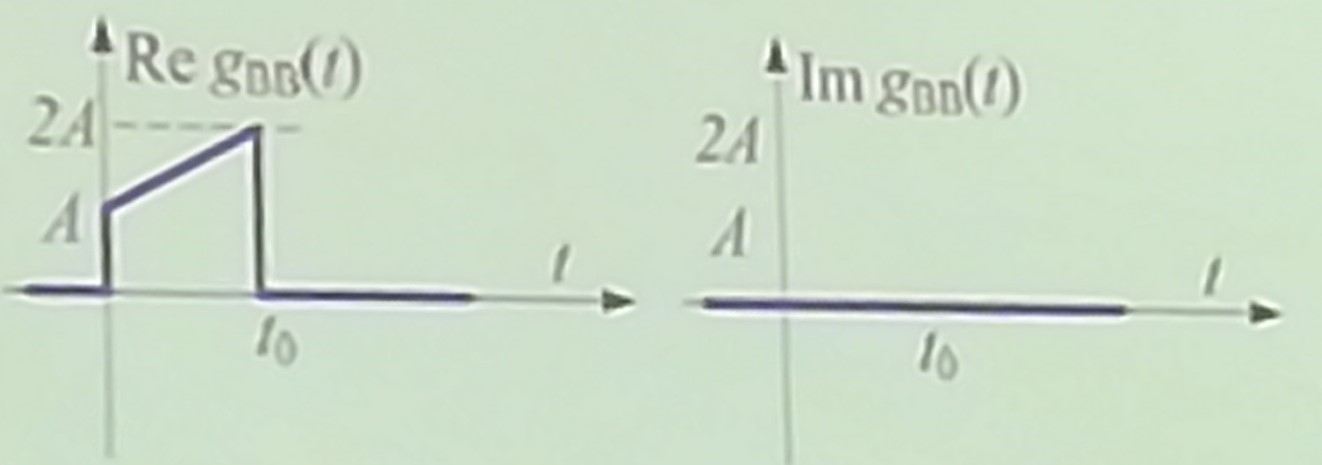
\includegraphics[width=10cm,height=3cm]{6.jpg}
\end{figure}
\section*{}
 (1)求等效基带信道的冲激响应。\\
(2)推导并画出在等效基带上的匹配滤波器(要求满足因果律)时域响应,并给出对应的最佳采样时刻。\\
7.某AWGN信道(信号增益为1)中的基带线性传输系统。为了保证采样点无失真,采用了升余弦滚降设计,
滚降系数0.5,调制符号率$R_s=1Msps$,采用双极性传输,电平序列独立。\\
(1)画出发送信号功率谱(标出关键频率)。\\
(2)画出接收匹配滤波器频响(标出关键频率)。\\
(3)求该系统在高信噪比时的频谱效率。\\
(4)当噪声单边功率谱密度$n_0=1\mu W/Hz$,信号功率为50mW,求该系统的最小误符号率(近似值)。判决
出来的平均每比特包含源发送序列的多少信息?\\
(5)在前一小题的条件基础上,若在接收机暂不判决,根据判决前(注意不是判决后)的采样电平序列,可以得
到的关于发端信源的信息量的速率为多少(近似值)。\\
8.某AWGN信道中的基带线性传输系统,为了保证采样点无失真,采用了升余弦滚降设计,滚降系数为0.5,调
制符号率为$R_s=1Msps$。信源为独立比特流,增加采取了以下措施。每个比特先映射为正负为$A$的电平,
得到电平序列$\{b_n\}$,然后将相邻两个电平相加得到一个新的电平序列$\{a_n\}$。其中$a_n=b_n+b_
  {n-1}$,将新得到的电平序列$\{a_n\}$。作为待传电平序列,进行基带成形发送。推导出发送信号功率谱
表达式,并画出功率谱。\\

\end{document}
